% =============================================================================
% SECTION 3: METHODOLOGY
% =============================================================================
\section{Proposed Methodology}

This section presents the six-stage pipeline model (Section~3.1), the build and test platform that implements it (Section~3.2), and the stage-aware detection methodology built on the same decomposition (Section~3.3).
The first two are implemented and evaluated in this paper; the third is proposed, with rule development and empirical validation scoped as future work.

% -----------------------------------------------------------------------------
\subsection{The Six-Stage Pipeline Model}
% -----------------------------------------------------------------------------

\subsubsection{Decomposition and Notation}

We model a shellcode loader as a sequence of six functional stages that share a mutable context.
The stages are Anti-Analysis (L0), Storage (L1), Allocation (L2), Transformation (L3), Writing (L4), and Execution (L5).
Fig.~\ref{fig:pipeline} summarizes the pipeline and the data that flows between stages.

\begin{figure}[htbp]
    \centering
    \setlength{\fboxsep}{8pt}
    \fbox{\parbox{0.9\columnwidth}{
    \centering
    \small
    \texttt{L0: Anti-Analysis}\\
    $\downarrow$ \textit{(environment validated)}\\[2pt]
    \texttt{L1: Storage} $\rightarrow$ \textit{encrypted data, key}\\
    $\downarrow$\\[2pt]
    \texttt{L2: Allocation} $\rightarrow$ \textit{target memory region}\\
    $\downarrow$\\[2pt]
    \texttt{L3: Transformation} $\rightarrow$ \textit{decrypted shellcode}\\
    $\downarrow$\\[2pt]
    \texttt{L4: Writing} $\rightarrow$ \textit{shellcode in memory}\\
    $\downarrow$\\[2pt]
    \texttt{L5: Execution} $\rightarrow$ \textit{control transfer}
    }}
    \caption{The six-stage pipeline. Each stage has a defined responsibility and extends the shared context that subsequent stages consume.}
    \label{fig:pipeline}
\end{figure}

Stages run sequentially and communicate through a shared context $\sigma$ that accumulates encrypted payload data, cryptographic material, allocation pointers, decrypted shellcode, and process handles as execution progresses.
If any stage returns failure, the loader aborts and later stages are skipped.

We identify each technique as $L_i.T_j$, where $i$ is the stage index and $j$ indexes techniques within that stage.
A complete loader configuration is therefore a tuple

\begin{equation}
    C = (L_0.T_a,\ L_1.T_b,\ L_2.T_c,\ L_3.T_d,\ L_4.T_e,\ L_5.T_f),
    \label{eq:config}
\end{equation}

\noindent which provides an unambiguous label for describing and comparing loader variants throughout the paper.

\subsubsection{Stage Definitions}

\textit{L0 --- Anti-Analysis.}
Performs environment checks such as debugger detection, sandbox evasion, and timing checks, and aborts the loader if indicators are found.
The stage is optional and produces no output consumed by later stages.

\textit{L1 --- Storage.}
Defines how the shellcode is held and retrieved: embedded in the binary (for example, in the \texttt{.rdata} section), read from disk, or fetched from a remote server.
Its output is the encrypted payload and the associated cryptographic material.

\textit{L2 --- Allocation.}
Prepares the memory region that will hold the shellcode, for example via \texttt{VirtualAlloc} locally or \texttt{VirtualAllocEx} in a remote process.
The permission profile---RWX in one step, or RW followed by a later flip to RX---is part of the technique choice and interacts with L4.

\textit{L3 --- Transformation.}
Converts the stored payload into executable bytes.
Options range from no transformation (plaintext) to strong encryption such as AES-128-CTR.
This stage is the main determinant of static-signature evasion.

\textit{L4 --- Writing.}
Places the transformed shellcode into the allocated region, either locally via \texttt{memcpy} or cross-process via \texttt{WriteProcessMemory}.
When paired with an RW-only allocation in L2, this stage also flips the protection to RX.

\textit{L5 --- Execution.}
Transfers control to the shellcode.
Techniques include thread creation (\texttt{CreateThread}), callback abuse (for example \texttt{EnumDisplayMonitors}), fibers (\texttt{CreateFiber} followed by \texttt{SwitchToFiber}), APC queuing, and process hollowing.

\subsubsection{Shared Context and API Abstraction}

All stages communicate through a shared \texttt{TechniqueContext} structure that carries the encrypted payload and length, cryptographic key and nonce, the decrypted-shellcode buffer, the allocated-memory pointer, and a target process handle for remote injection.

Orthogonal to the pipeline, an API abstraction layer determines how Windows system calls are invoked.
The platform supports two modes: (i) standard Windows API through \texttt{kernel32} and \texttt{ntdll}, and (ii) direct syscalls through custom assembly stubs that issue the \texttt{syscall} instruction with system service numbers resolved dynamically from a loaded \texttt{ntdll}.
The API mode applies to stages L2, L4, and L5, which lets us evaluate the effect of API invocation style independently from stage technique selection.

\subsubsection{Stage Interactions: the W\texorpdfstring{$^{\wedge}$}{\textasciicircum}X Pattern}
\label{sec:wxpattern}

Although stages are defined with independent responsibilities, some technique choices in different stages are coupled, and the coupling carries detection implications that are central to the analysis in later sections.
The clearest example is the pairing of L2 and L4, which jointly determine the memory-protection profile of the shellcode buffer.

Two valid pairings are implemented:

\begin{itemize}[leftmargin=*, itemsep=2pt]
    \item \textit{Single-step RWX}: (\texttt{T2.1}, \texttt{T4.1}).
    L2 allocates with \texttt{PAGE\_EXECUTE\_READWRITE}; L4 copies the shellcode with \texttt{memcpy}.
    The buffer is writable and executable at the same time.

    \item \textit{Two-step W$^{\wedge}$X}: (\texttt{T2.2}, \texttt{T4.2}).
    L2 allocates with \texttt{PAGE\_READWRITE}; L4 copies the shellcode and then flips the protection to \texttt{PAGE\_EXECUTE\_READ} via \texttt{VirtualProtect}.
    At no point is the buffer both writable and executable.
\end{itemize}

Both pairings produce the same end-state functionality---the shellcode executes in both cases---but they differ in the telemetry they generate.
The first pairing produces a single allocation event with an RWX protection mask, which is a well-established heuristic signal for suspicious memory preparation.
The second pairing produces an initial RW allocation (benign-looking in isolation) followed by a \texttt{VirtualProtect} call that flips the region to executable; this latter sequence is also observable, but it overlaps with patterns used by legitimate JIT compilers and some packers, so a signature-only rule targeting it is noisier.
Section~3.3 captures the two as separate entries in the detection surface for L2 and L4.

Other stage pairs show weaker but non-zero coupling.
The L3 choice affects both the payload size that L4 writes and the entropy visible to static scans targeting L1.
The L5 choice affects the API trace generated around L4 when writing and execution occur in the same process versus across processes.
These couplings motivate comparing loader variants as complete tuples $C$ rather than one stage at a time.

% -----------------------------------------------------------------------------
\subsection{Build and Test Platform}
% -----------------------------------------------------------------------------

The platform implements the pipeline model through three components that operate end-to-end, from a single CLI invocation to a detection verdict.
Figure~\ref{fig:platform} summarizes the workflow.

\begin{figure*}[t]
    \centering
    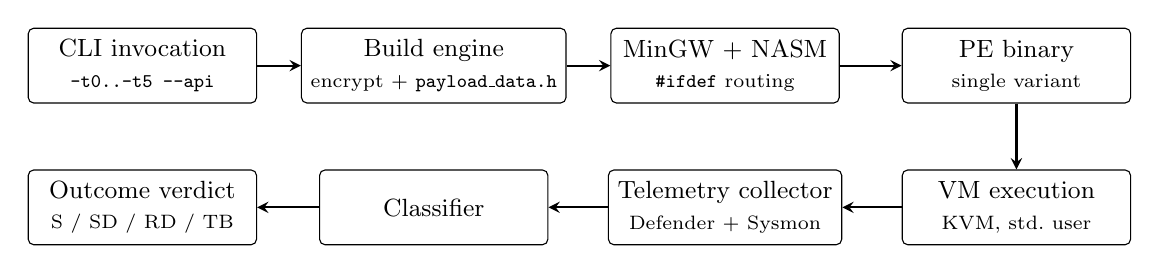
\begin{tikzpicture}[
        box/.style={draw, rounded corners=2pt, align=center, font=\small,
                    minimum height=0.95cm, minimum width=2.9cm},
        arr/.style={->, >=stealth, thick}
    ]
    \node[box] (cli) at (0,1.3)    {CLI invocation\\\scriptsize \texttt{-t0..-t5 --api}};
    \node[box] (py)  at (3.7,1.3)  {Build engine\\\scriptsize encrypt + \texttt{payload\_data.h}};
    \node[box] (cc)  at (7.4,1.3)  {MinGW + NASM\\\scriptsize \texttt{\#ifdef} routing};
    \node[box] (bin) at (11.1,1.3) {PE binary\\\scriptsize single variant};

    \node[box] (vm)  at (11.1,-0.5) {VM execution\\\scriptsize KVM, std.\ user};
    \node[box] (col) at (7.4,-0.5)  {Telemetry collector\\\scriptsize Defender + Sysmon};
    \node[box] (cls) at (3.7,-0.5)  {Classifier};
    \node[box] (out) at (0,-0.5)    {Outcome verdict\\\scriptsize S / SD / RD / TB};

    \draw[arr] (cli) -- (py);
    \draw[arr] (py)  -- (cc);
    \draw[arr] (cc)  -- (bin);
    \draw[arr] (bin) -- (vm);
    \draw[arr] (vm)  -- (col);
    \draw[arr] (col) -- (cls);
    \draw[arr] (cls) -- (out);
    \end{tikzpicture}
    \caption{End-to-end platform workflow. A single CLI invocation drives build, execution in an isolated VM, telemetry collection, and outcome classification, producing one $(C, \text{outcome})$ pair per run.}
    \label{fig:platform}
\end{figure*}

\subsubsection{Build Engine}

User-specified technique choices are mapped to C/C++ preprocessor flags by a definitions module.
A typical invocation is:

\begin{lstlisting}[basicstyle=\ttfamily\scriptsize, numbers=none, frame=none]
python cli.py -s payload.bin \
  -t0 antidebug -t1 rdata -t2 local_rw \
  -t3 aes -t4 local_rx -t5 fiber \
  --api syscalls
\end{lstlisting}

Each technique is a self-contained header file with a single \texttt{inline} function, selected at compile time by its preprocessor flag.
The build engine encrypts the shellcode according to the L3 choice, generates a C byte array in a \texttt{payload\_data.h} header, and invokes the MinGW-w64 cross-compiler to produce a standalone Windows PE executable.

Because stage selection is resolved at preprocessor time, each output binary contains only the selected technique code.
There is no runtime dispatch table or reflection logic that could itself become a detection signal, which keeps each variant as close as possible to a hand-written loader for that specific configuration.

\subsubsection{VM Orchestrator}

Each build is tested in an isolated Windows VM backed by KVM and libvirt.
The snapshots used for evaluation include Windows Defender with definitions updated at test time and Sysmon with a loader-oriented configuration.
A test run automates: snapshot revert, VM start, payload transfer over an internal network, C2 listener setup on the host, payload execution under a standard user account, telemetry collection with elevated credentials, and VM shutdown.

\subsubsection{Telemetry and Outcome Classification}

A PowerShell collector gathers Windows Defender events (IDs 1116, 1117, and 1118) and the Sysmon events most relevant to loader behavior: event~8 (CreateRemoteThread) for L5, event~10 (ProcessAccess) for L2 and L4, event~11 (FileCreate) for L1, and event~25 (ProcessTampering) for process hollowing.
The collector emits both human-readable text and stage-annotated CSV so that results can be aggregated across runs.

We classify each test run into one of four outcomes: \textit{Success} (callback received), \textit{Transfer Blocked} (deleted during file transfer), \textit{Static Detection} (deleted before execution), or \textit{Runtime Detection} (blocked during execution).

% -----------------------------------------------------------------------------
\subsection{Stage-Aware Detection Methodology (Proposed)}
% -----------------------------------------------------------------------------

The pipeline model is also intended to serve as a scaffolding for detection engineering.
This subsection describes the methodology we propose for that purpose.
Rule implementation and empirical validation of the methodology are scoped as future work (Section~5.5); this paper presents its design only.

\subsubsection{Detection Surface Mapping}

Each stage produces characteristic side effects that are observable through specific telemetry sources.
Table~\ref{tab:detection_surface} maps each stage to its candidate detection phase, telemetry sources, and observable indicators.
The intent is that, once these candidates are turned into concrete rules, the table identifies where in the pipeline each rule would gain visibility.

\begin{table*}[htbp]
    \centering
    \caption{Proposed detection surface per pipeline stage. For each stage we list a candidate detection phase, telemetry sources, and observable indicators. Entries describe where rules could be placed; concrete rule bodies are left to future work.}
    \label{tab:detection_surface}
    \small
    \begin{tabular}{@{}p{1.8cm}p{3.0cm}p{4.5cm}p{5.7cm}@{}}
        \toprule
        \textbf{Stage} & \textbf{Detection Phase} & \textbf{Telemetry Sources} & \textbf{Observable Indicators} \\
        \midrule
        L0: Anti-Analysis &
        Behavioral heuristics &
        ETW tracing~\cite{etw}, API call logs &
        Timing anomalies; queries to \texttt{IsDebuggerPresent}; unusual API call sequences before functional activity \\
        \midrule
        L1: Storage &
        Static scan, network &
        AV scan, Sysmon~\cite{sysmon} Event 11 (FileCreate), Event 3 (NetworkConnect) &
        High-entropy embedded sections; network connections to unknown servers for payload retrieval \\
        \midrule
        L2: Allocation &
        Memory monitoring &
        Sysmon Event 10 (ProcessAccess), ETW Kernel-Memory &
        RWX allocation from non-system process; cross-process allocation via \texttt{VirtualAllocEx} \\
        \midrule
        L3: Transform. &
        Static / entropy &
        YARA rules, PE analysis &
        High-entropy data sections; cryptographic constants (S-boxes); decrypted content matching known signatures \\
        \midrule
        L4: Writing &
        Memory modification &
        Sysmon Event 10, kernel callbacks &
        \texttt{WriteProcessMemory} targeting executable regions; large writes to RWX pages \\
        \midrule
        L5: Execution &
        Thread / callback &
        Sysmon Event 8 (CreateRemoteThread), ETW thread events &
        Thread start address in non-image memory; callback to dynamically allocated regions \\
        \bottomrule
    \end{tabular}
\end{table*}

\textbf{Visibility caveat: process locality.}
The mapping above is technique-source-dependent and process-boundary-dependent.
For a loader whose L2, L4, and L5 operations all execute inside a single process, intra-stage technique choices---for example local thread creation versus callback-based execution versus fiber switching at L5---do not surface as distinct Sysmon events because the underlying operations either lack a dedicated event (\texttt{VirtualProtect}, \texttt{SwitchToFiber}) or do not cross a process boundary (\texttt{CreateThread} on the calling process).
Once a stage crosses the process boundary, the dedicated cross-process events (Event~8 \texttt{CreateRemoteThread}, Event~10 \texttt{ProcessAccess} with cross-image source/target, Event~25 \texttt{ProcessTampering}) fire and Sysmon attribution becomes per-technique.
Distinguishing intra-process technique choices therefore requires telemetry sources beyond Sysmon, such as ETW Kernel-Memory providers, AMSI, or memory-scan callbacks; the methodology accommodates this by treating telemetry source as a per-stage parameter of the mapping rather than fixing it to one provider.

\subsubsection{Proposed Technique-to-Rule Function}

We formalize the intended relationship between techniques and detection rules as a mapping

\begin{equation}
    D: L_i.T_j \rightarrow \{(s_k, o_k, r_k)\},
    \label{eq:detection_map}
\end{equation}

\noindent that associates each technique with tuples of telemetry source $s_k$ (for example, a Sysmon event ID), observable indicator $o_k$, and detection rule $r_k$ (Sigma or YARA).
Once populated, $D$ would support two operations.
First, \textit{coverage checking} verifies that every technique $L_i.T_j$ implemented in the platform has at least one tuple in $D$; an empty image indicates a blind spot.
Second, \textit{gap identification} compares the telemetry collected by the platform for each run against the rules referenced by $D$; a run where a rule should have fired but did not points to a concrete rule defect.
Populating $D$ with rule bodies and running them against the platform's telemetry is the planned empirical validation.

\subsubsection{Layered Defense View}

The detection surface in Table~\ref{tab:detection_surface} suggests four natural defense layers aligned with the pipeline:

\begin{itemize}[leftmargin=*, itemsep=1pt]
    \item \textit{Static analysis} (L1, L3): signature matching and entropy analysis on disk; effective against weak or absent transformation.
    \item \textit{API monitoring} (L2, L4, L5): tracing system calls for allocation, writing, and execution; weakened by direct syscalls.
    \item \textit{Behavioral analysis} (L0, L5): analyzing timing, call sequences, and callback abuse; largely independent of API hooking.
    \item \textit{Memory forensics} (L3, L4): scanning in-memory content after decryption; orthogonal to encryption strength.
\end{itemize}

A defense program covering all four layers is harder to bypass than one that relies on a single layer, because an attacker can select techniques at each stage that individually defeat any one layer.
This observation is a motivation for the stage-level framing; validating it with real rules is part of the future work.
